\chapter{2011}
\label{cha:2011}

\section{Primera parte}
\label{sec:primera-parte}

\begin{Problema}{1}
  Cuando Esteban naci\'o, su pap\'a ten\'ia $28$ a\~nos. Si ahora
  Esteban tiene una tercio de la edad de su pap\'a, ?`cu\'antos a\~nos
  tiene Esteban?

  \begin{inparaenum}
  \item $7$ \esp
  \item $9$ \esp
  \item $14$ \esp
  \item $17$ \esp
  \item \nota
  \end{inparaenum}
\end{Problema}

\begin{Solucion}
  
\end{Solucion}

\begin{Problema}{2}
  En la terminal de autobuses de Xicotl\'an de las Flores sale un
  autob\'us de la L\'inea A cada 9 minutos a partir de las 6:00 AM, un
  autob\'us de la L\'inea B cada 13 minutos a partir de las 7:00 AM y
  un autob\'us de la L\'inea C cada 11 minutos a partir de las 8:00
  AM. ?`Cu\'antos autobuses de las l\'ineas A, B y C salen de la
  terminal desde las 6:00 AM y hasta las 5:00 PM?

  \begin{inparaenum}
  \item $151 $ \esp
  \item $154$ \esp
  \item $168 $ \esp
  \item $171$ \esp
  \item \nota
  \end{inparaenum}
\end{Problema}

\begin{Solucion}
  
\end{Solucion}

\begin{Problema}{3}
  ?` Cu\'ales son los dos \'ultimos d\'igitos del n\'umero $2011^{2011}$ ?

  \begin{inparaenum}
  \item $01$ \esp
  \item $11$ \esp
  \item $21$ \esp
  \item $91$ \esp
  \item \nota.
  \end{inparaenum}
\end{Problema}

\begin{Solucion}
  
\end{Solucion}

\begin{Problema}{4}
  Se escriben todos los n\'umeros del 1 al 1000. ?`Cu\'antas veces
  aparece el d\'igito $5$?

  \begin{inparaenum}
  \item $100$ \esp
  \item $200$ \esp
  \item $300$ \esp
  \item $333$ \esp
  \item \nota.
  \end{inparaenum}
\end{Problema}

\begin{Solucion}
  
\end{Solucion}

\begin{Problema}{5}
  Un torneo es de eliminaci\'on simple si cada partido se juega entre
  dos equipos y el equipo que pierde abandona el torneo.  Si en un
  torneo de eliminaci\'on simple (en el que no se permiten los
  empates) participan $1024$ equipos, ?`cu\'antos partidos se juegan
  para determinar al campe\'on?

  \begin{inparaenum}
  \item $10$ \esp
  \item $11$ \esp
  \item $1023$ \esp
  \item $1024$ \esp
  \item \nota.
  \end{inparaenum}
\end{Problema}

\begin{Solucion}
  
\end{Solucion}

\begin{Problema}{6}
  Un cuadrado de \'area $4$ est\'a inscrito en un tri\'angulo
  is\'osceles como se muestra en la figura. La distancia de un
  v\'ertice de la base del tri\'angulo al v\'ertice m\'as pr\'oximo
  del cuadrado es $1$. ?`Cu\'al es el \'area del tri\'angulo m\'as
  grande?

  \begin{center}
    %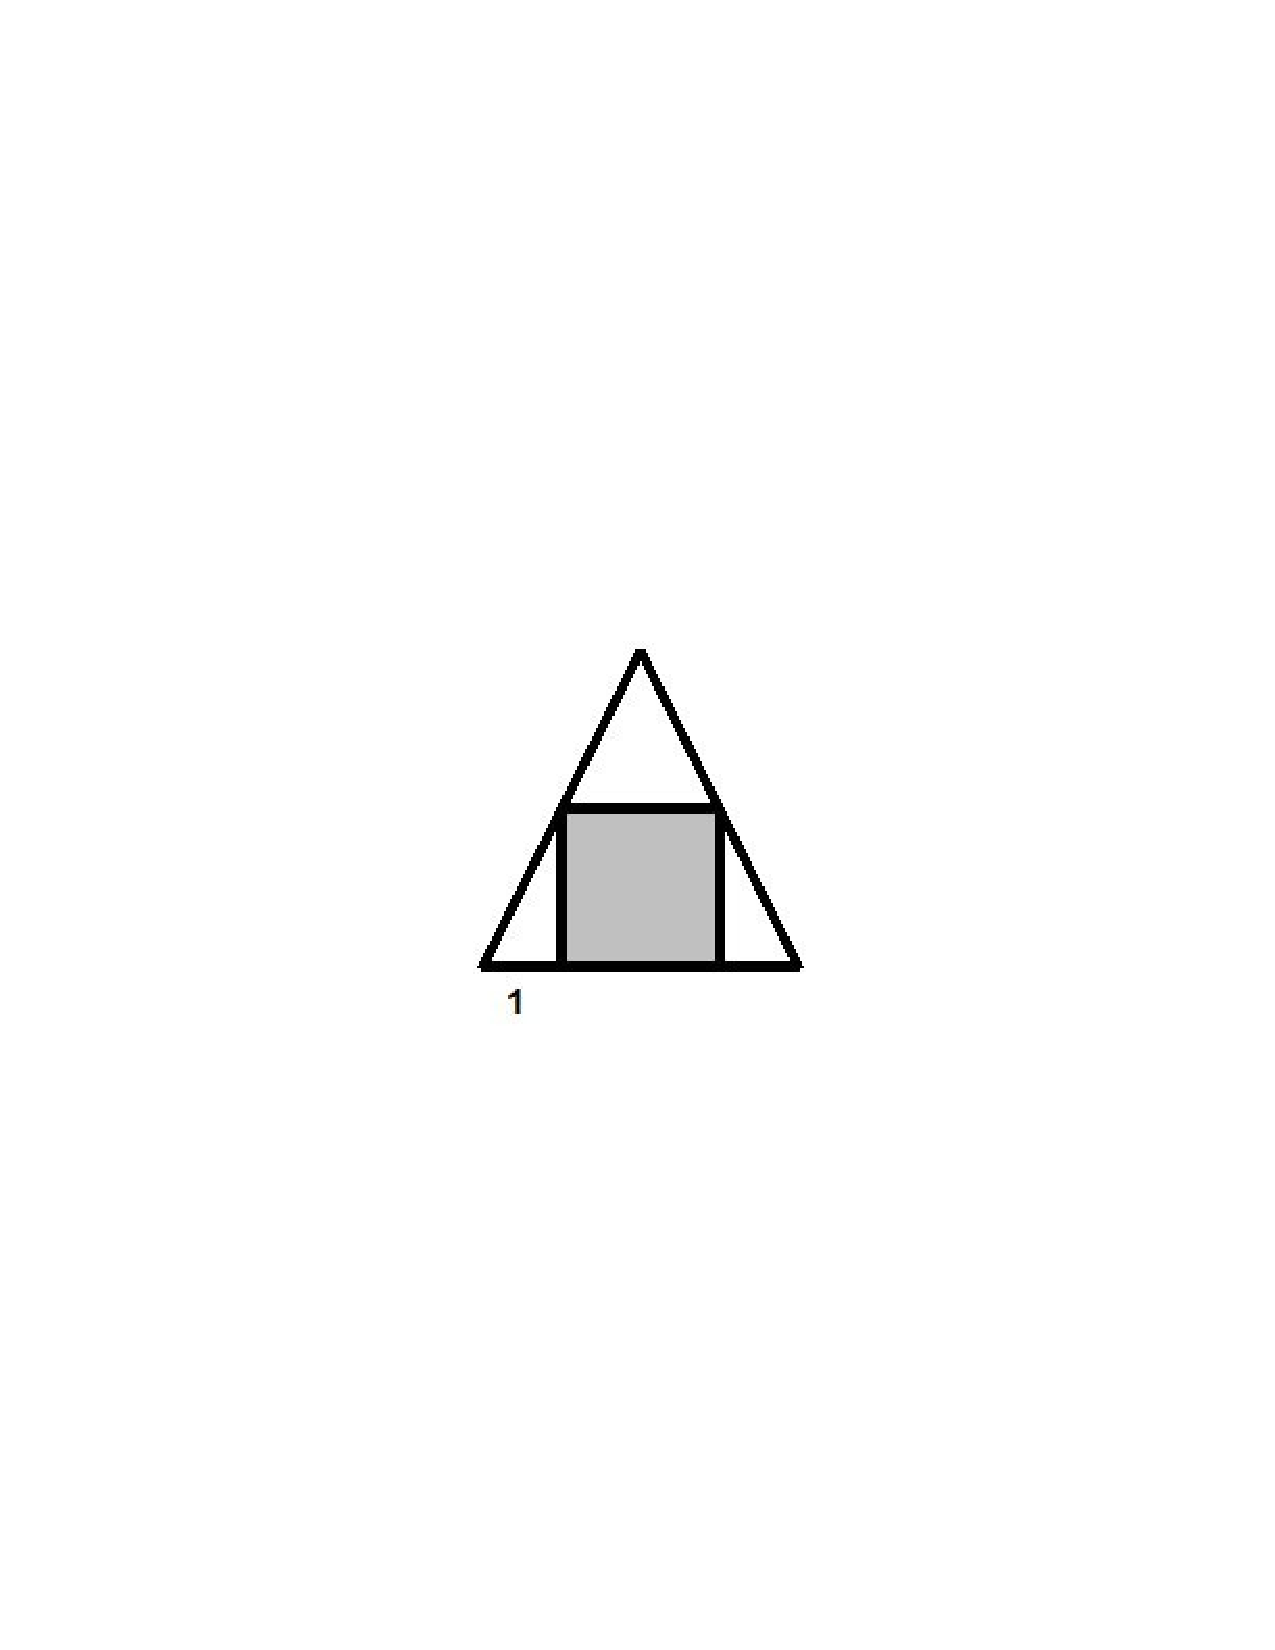
\includegraphics[scale=0.5,viewport=203 299 409 493]{triangulo_con_cuadrado.pdf}
  \end{center}

  \begin{inparaenum}
  \item $8$ \esp
  \item $10$ \esp
  \item $16$ \esp
  \item $24$ \esp
  \item \nota.
  \end{inparaenum}
\end{Problema}

\begin{Solucion}
  
\end{Solucion}

\begin{Problema}{7}
  Un cuadrado de \'area $16$ se divide en cuatro cuadrados iguales
  como se muestra en el dibujo. ?`Cu\'al es el \'area delimitada por
  la circunferencia que pasa por los centros de los cuatro cuadrados
  peque\~nos?

  \begin{center}
    %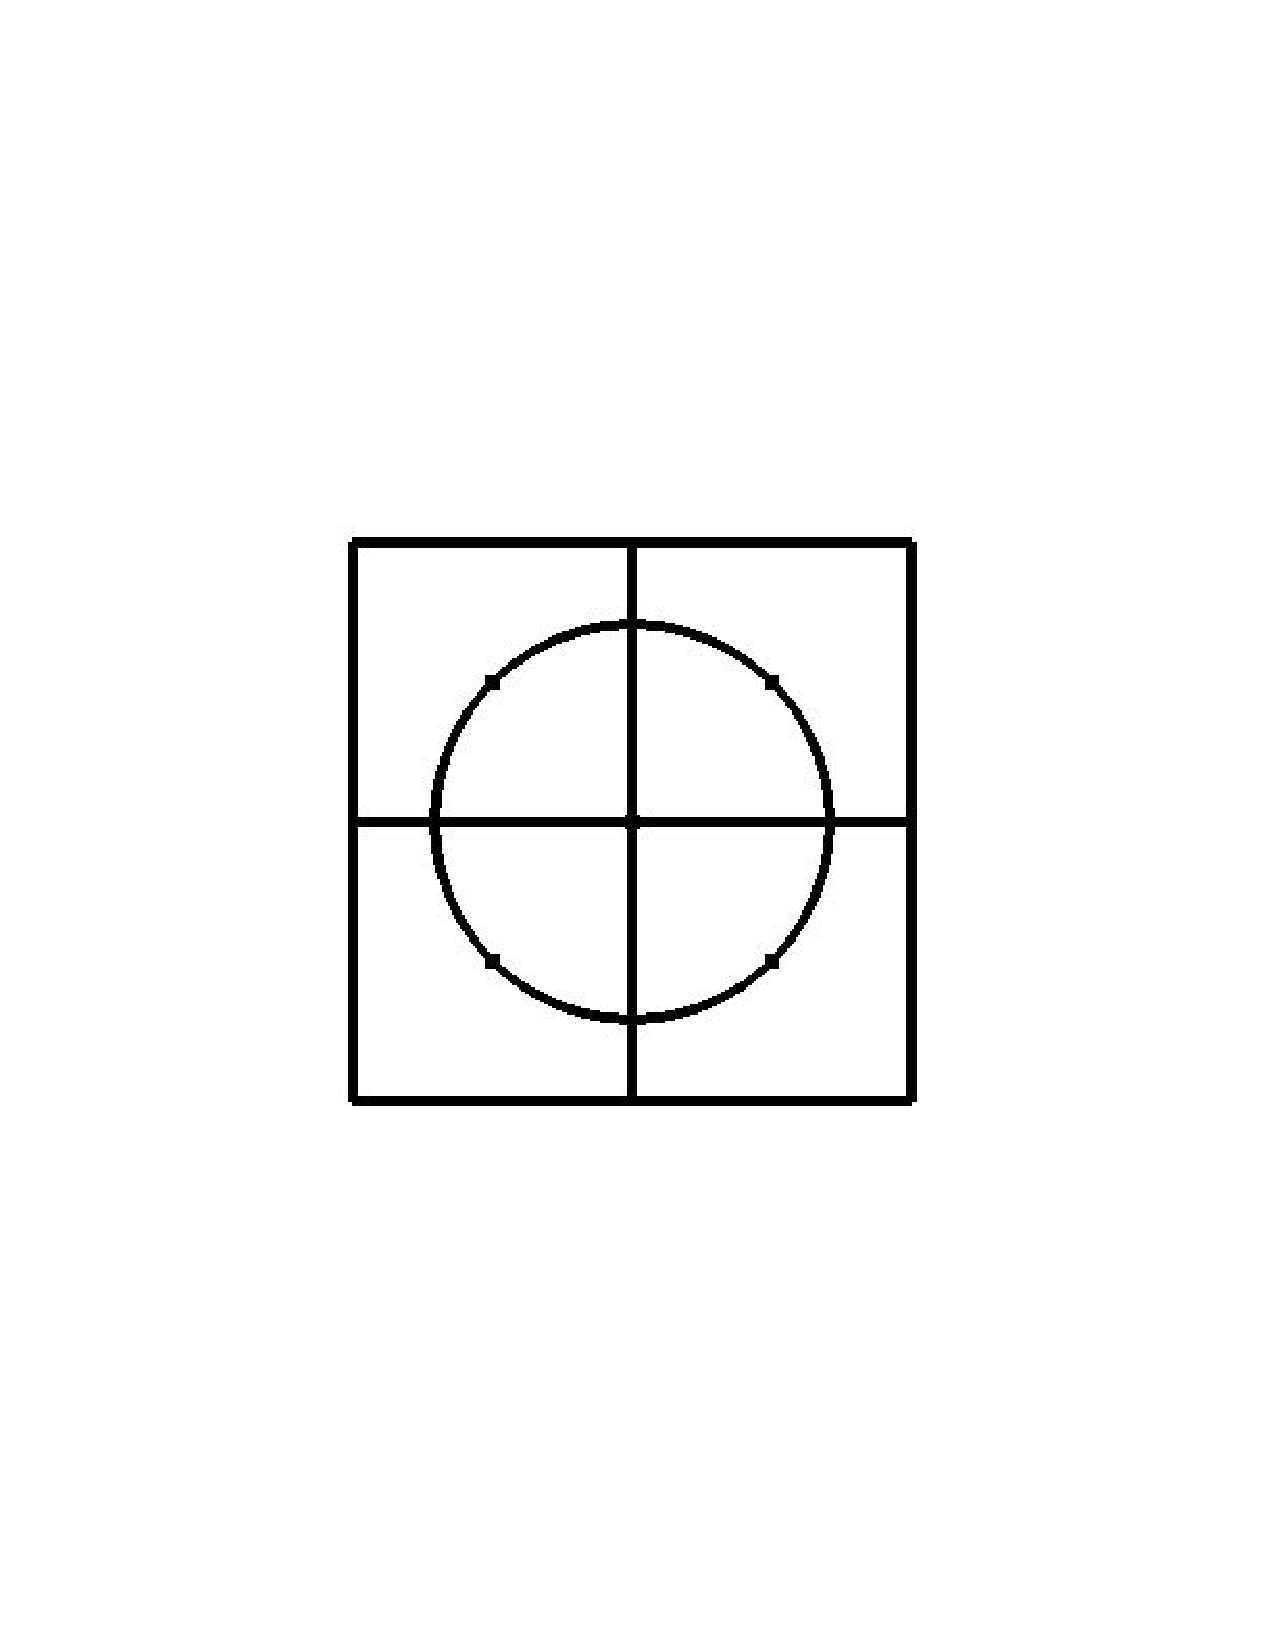
\includegraphics[scale=0.5,viewport=146 243 466 549]{cuadrado_con_circunferencia.pdf}
  \end{center}

  \begin{inparaenum}
  \item $\frac{\pi}{2}$ \esp
  \item $\pi$ \esp
  \item $2 \pi$ \esp
  \item $\pi^2$ \esp
  \item \nota.
  \end{inparaenum}
\end{Problema}

\begin{Solucion}
  
\end{Solucion}

\begin{Problema}{8}
  ?`Cu\'antos n\'umeros enteros mayores que $100$ y menores que
  $1000$ tienen la propiedad que la suma de sus d\'igitos es $13$?

  \begin{inparaenum}
  \item $39$ \esp
  \item $63$ \esp
  \item $69$ \esp
  \item $81$ \esp
  \item \nota.
  \end{inparaenum}
\end{Problema}

\begin{Solucion}
  
\end{Solucion}

\begin{Problema}{9}
  En un bote hay $100$ canicas de cada uno de $5$ diferentes
  colores. Se extraen las canicas de una a una sin ver. ?`Cu\'al es el
  m\'inimo n\'umero de canicas que se necesitan sacar para garantizar
  que hay al menos $10$ de un mismo color?

  \begin{inparaenum}
  \item $10$ \esp
  \item $11$ \esp
  \item $41$ \esp
  \item $55$ \esp
  \item \nota.
  \end{inparaenum}
\end{Problema}

\begin{Solucion}
  
\end{Solucion}

\begin{Problema}{10}
  En la siguiente figura los centros de las circunferencias interiores
  se encuentran sobre un di\'ametro de la circunferencia mayor y cada
  circunferencia toca a cada una de sus vecinas en un s\'olo punto.
  Sea $A$ el per\'imetro de la circunferencia mayor y sea $B$ la suma
  de los per\'imetros de las circunferencias sobre el di\'ametro de la
  circunferencia grande. ?`Cu\'al es la relaci\'on entre $A$ y $B$?

  \begin{center}
    %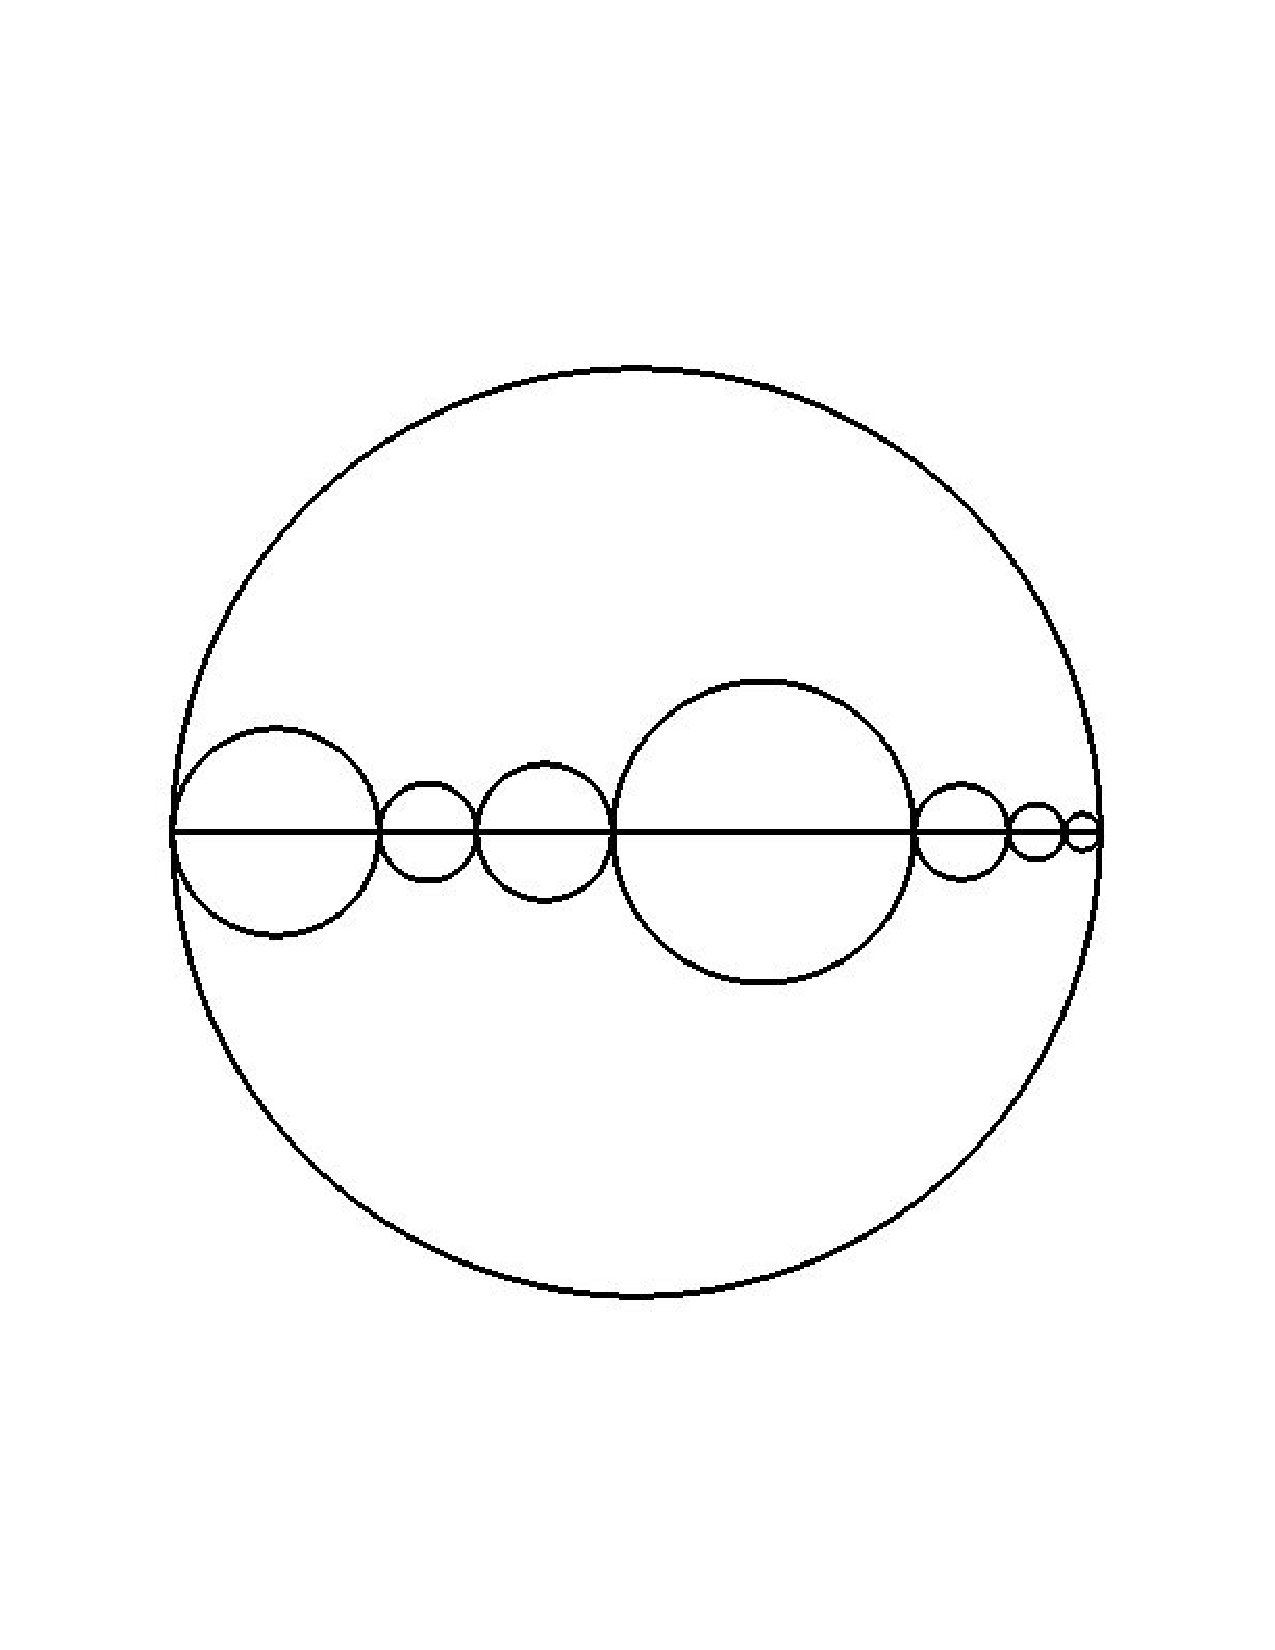
\includegraphics[scale=0.3,viewport=59 150 553 642]{circunferencias.pdf}
  \end{center}

  \begin{inparaenum}
  \item $A=2 B$ \espc
  \item $A=B$ \espc
  \item $2 A= B$ \espc
  \item $7 A = B$ \espc
  \item \nota.
  \end{inparaenum}
\end{Problema}

\begin{Solucion}
  
\end{Solucion}

\section{Segunda parte}
\label{sec:segunda-parte}

\begin{Problema}{11}
  Considera un tri\'angulo $ABC$ (es decir, el tri\'angulo con
  v\'ertices $A$, $B$ y $C$) y sea $M$ el punto medio del lado
  $AC$. Sea $P$ un punto cualquiera en el segmento $MB$. Demuestra que
  las \'areas de los tri\'angulos $APB$ y $CPB$ son iguales.
\end{Problema}

\begin{Solucion}
  
\end{Solucion}

\begin{Problema}{12}
  Una escalera de $10$ metros esta apoyada sobre una pared vertical de
  tal forma que el pie de la escalera se encuentra a $6$ metros de la
  pared. Un gato que est\'a subiendo por la escalera se encuentra a
  una distancia de $7$ metros de la base de la pared. ?`Qu\'e
  distancia le falta al gato para llegar a la cima de la escalera?

  \begin{center}
    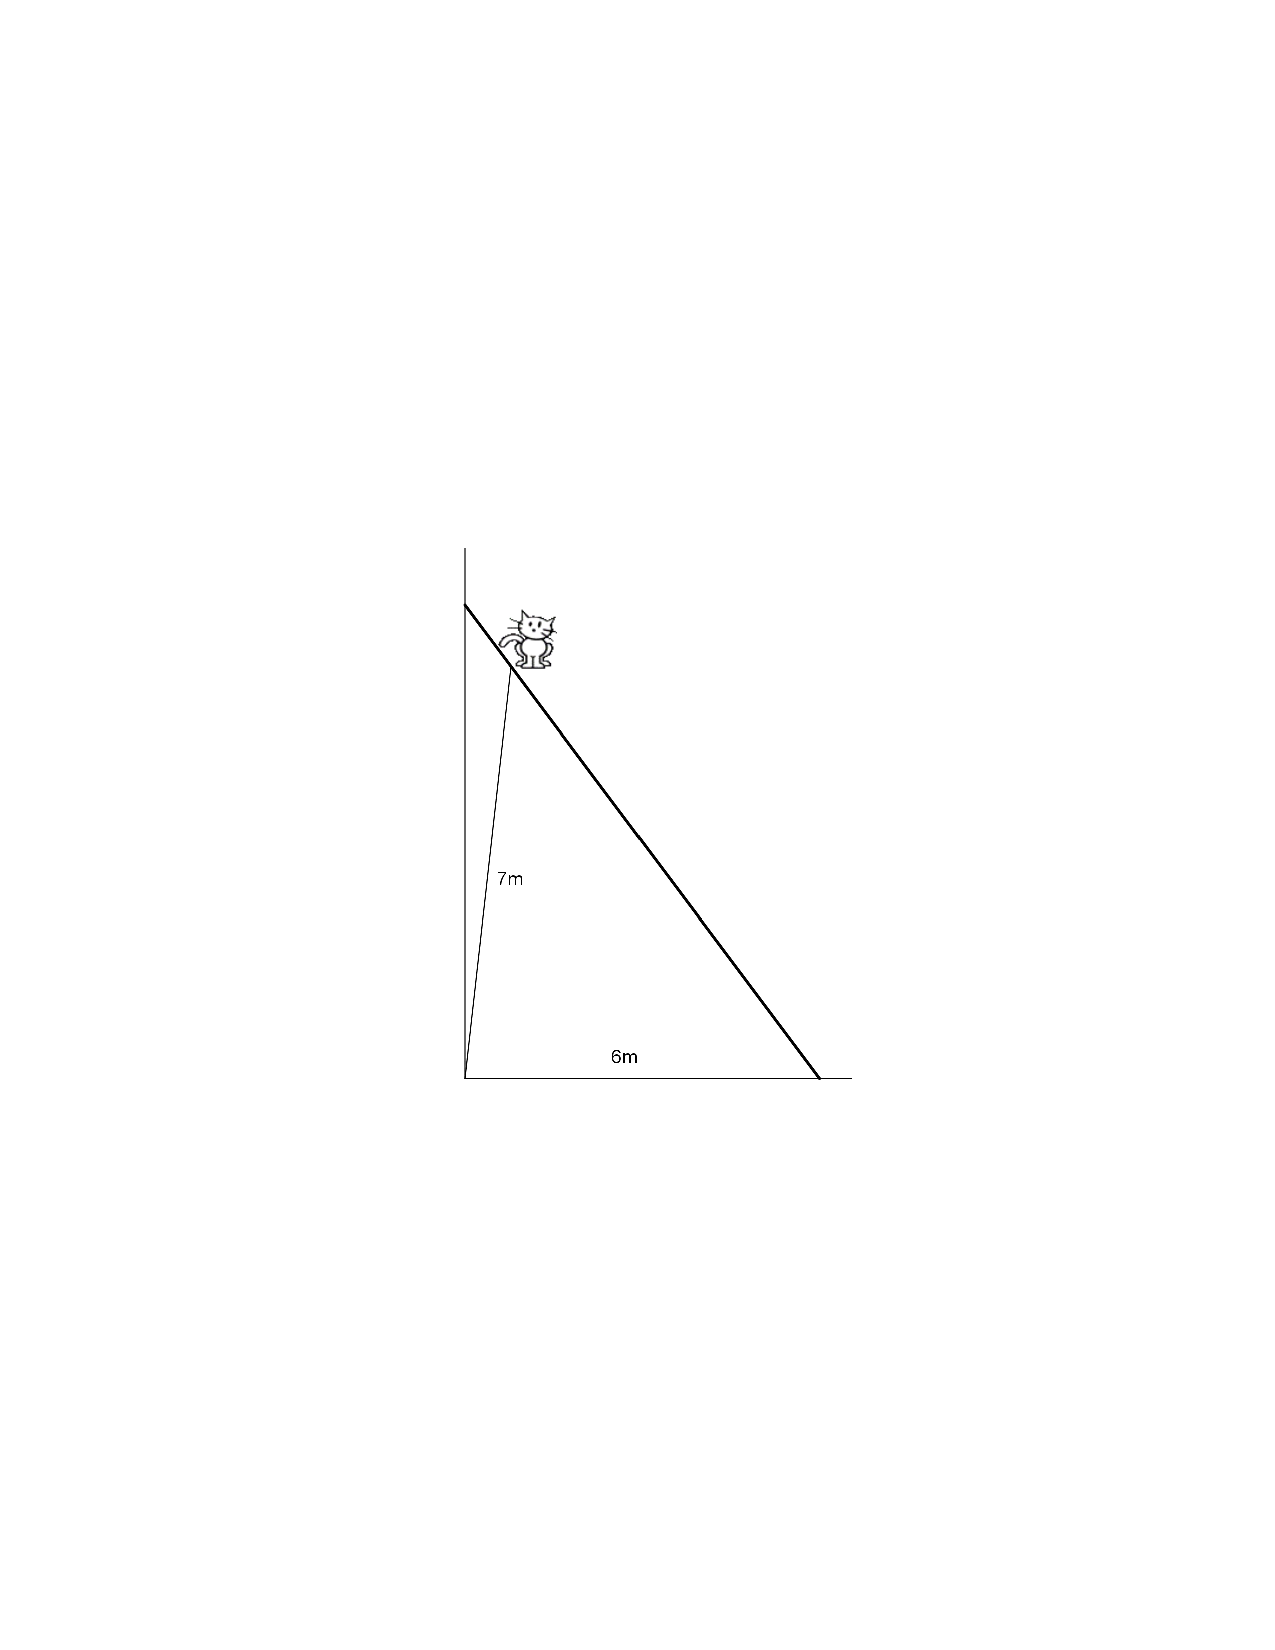
\includegraphics[scale=0.7,viewport=203 273 409 529]{gato.pdf}
  \end{center}
\end{Problema}

\begin{Solucion}
  
\end{Solucion}

\begin{Problema}{13}
  Una cuadr\'icula de $2011 \times 2011$ se llena escribiendo la
  palabra ``HIDALGO", una letra por cada casilla, en el orden que se
  indica en la figura. ?`Cu\'antas veces aparece la letra ``H'' en la
  primera columna (la que est\'a m\'as a la izquierda) de la
  cuadr\'icula?

  \begin{center}
    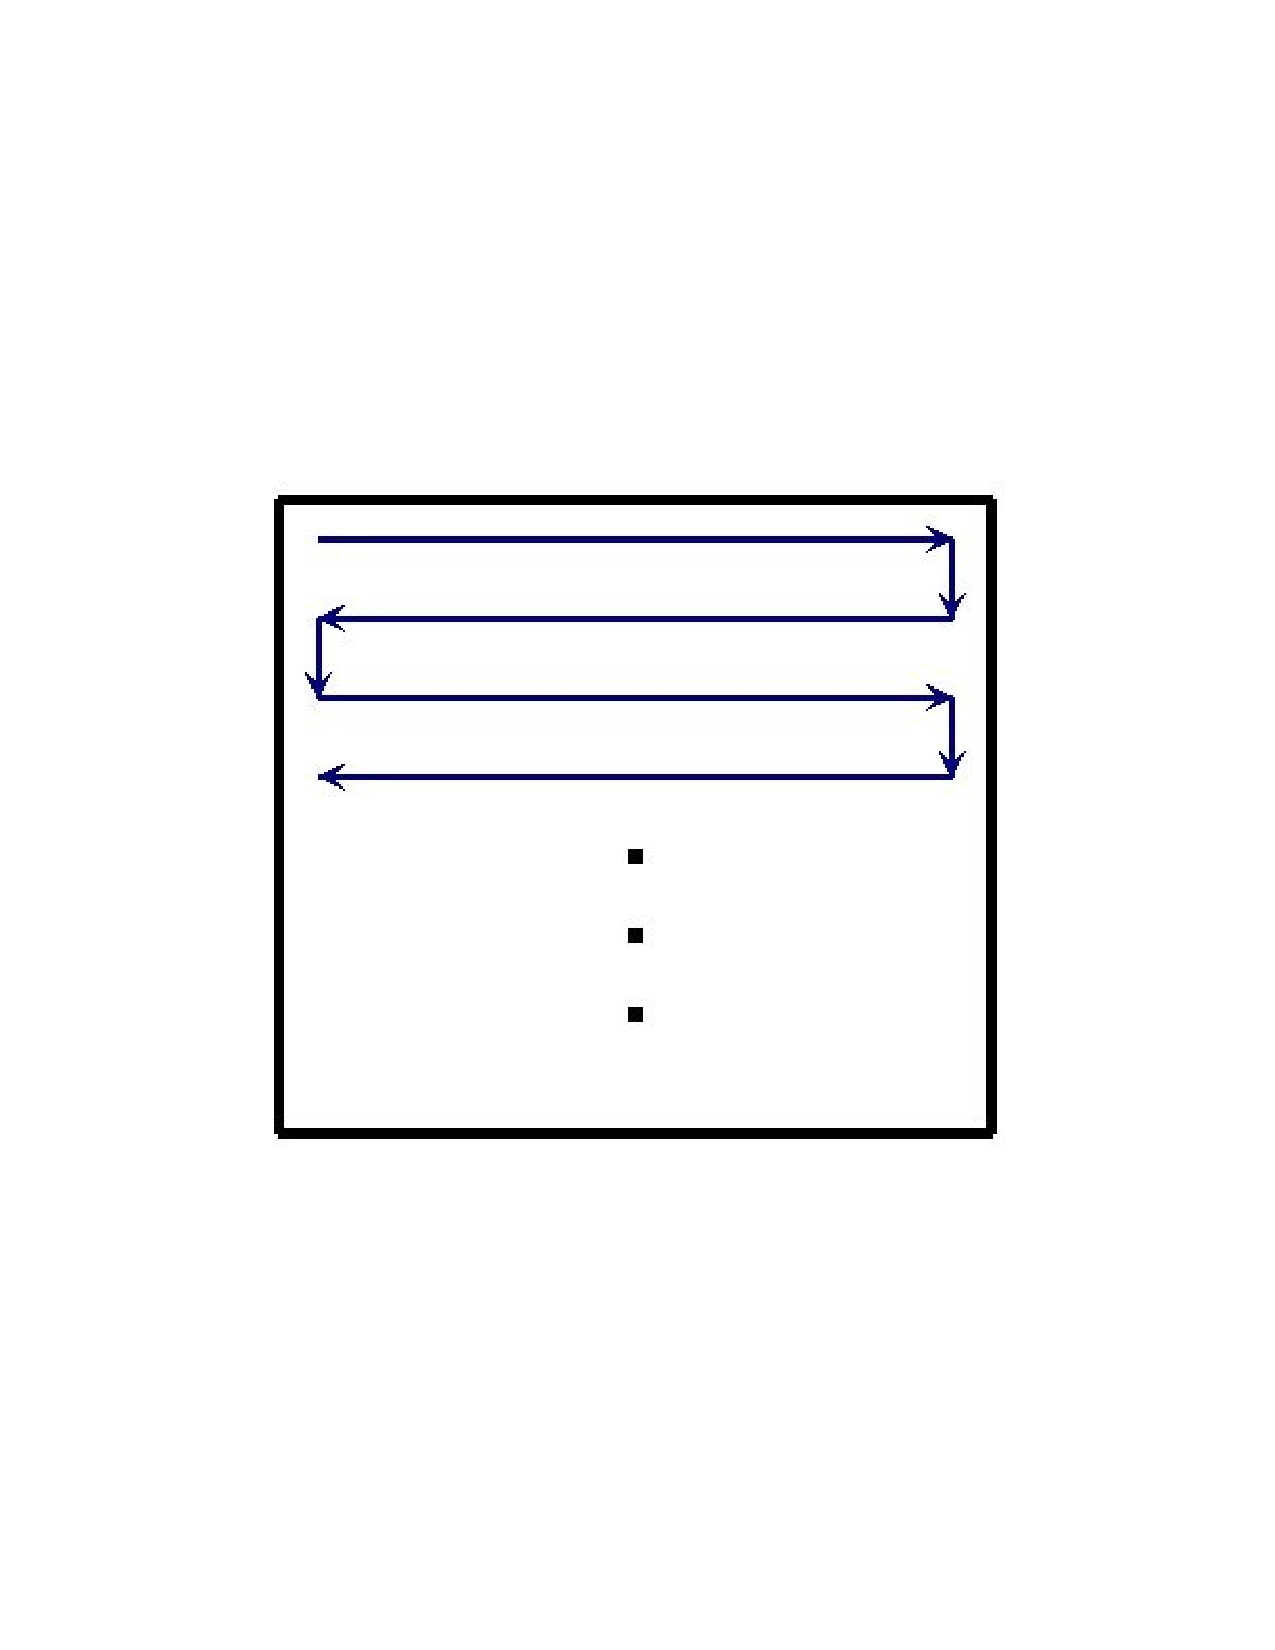
\includegraphics[scale=0.5,viewport=114 222 498 570]{direcciones.pdf}
  \end{center}
\end{Problema}

\begin{Solucion}
  
\end{Solucion}



%%% Local Variables: 
%%% mode: latex
%%% TeX-master: "libro"
%%% End: 